\documentclass[12pt,a4paper]{article}

% ---- Encoding & Language ----
\usepackage[utf8]{inputenc}
\usepackage[T1]{fontenc}
\usepackage[brazil]{babel}

% ---- Geometry (ABNT-like margins) ----
\usepackage[a4paper,top=3cm,bottom=2cm,left=3cm,right=2cm]{geometry}

% ---- Font ----
\usepackage{mathptmx}   % Times New Roman

% ---- Math ----
\usepackage{amsmath}
\usepackage{amssymb}

% ---- Graphics & Floats ----
\usepackage{graphicx}
\graphicspath{{figures/}{./figures/}{./}}
\usepackage{float}
\usepackage[labelfont=bf,font=small]{caption}
\usepackage{subcaption}

% ---- Tables ----
\usepackage{booktabs}
\usepackage{array}
\usepackage{tabularx}

% ---- Colors ----
\usepackage{xcolor}
\definecolor{unifblue}{RGB}{30,73,101}

% ---- Spacing ----
\usepackage{setspace}
\onehalfspacing
\setlength{\parindent}{1.25cm}
\usepackage{indentfirst}

% ---- Headers & Footers ----
\usepackage{fancyhdr}
\pagestyle{fancy}
\fancyhf{}
\fancyhead[L]{\footnotesize\textit{Tema~4 --- Process Mining $|$ Grupo~G5 --- UNIFESSPA}}
\fancyhead[R]{\footnotesize\thepage}
\renewcommand{\headrulewidth}{0.4pt}
\fancypagestyle{plain}{%
  \fancyhf{}
  \fancyhead[R]{\footnotesize\thepage}
  \renewcommand{\headrulewidth}{0pt}
}

% ---- Section formatting ----
\usepackage{titlesec}
\titleformat{\section}{\large\bfseries\color{unifblue}}{}{0em}{\thesection\quad}[\vspace{-4pt}\textcolor{unifblue}{\rule{\linewidth}{0.6pt}}]
\titleformat{\subsection}{\normalsize\bfseries}{}{0em}{\thesubsection\quad}
\titleformat{\subsubsection}{\normalsize\itshape}{}{0em}{\thesubsubsection\quad}

% ---- Lists ----
\usepackage{enumitem}
\setlist[itemize]{topsep=2pt,itemsep=1pt,parsep=0pt}
\setlist[enumerate]{topsep=2pt,itemsep=1pt,parsep=0pt}

% ---- Hyperlinks ----
\usepackage[hidelinks,colorlinks=false]{hyperref}

% ---- Misc ----
\usepackage{microtype}

% ===========================================================
\begin{document}
% ===========================================================

% -----------------------------------------------------------
% CAPA
% -----------------------------------------------------------
\begin{titlepage}
\centering
\vspace*{0.5cm}

{\large\bfseries UNIVERSIDADE FEDERAL DO SUL E SUDESTE DO PARÁ --- UNIFESSPA}\\[0.25cm]
{\normalsize Instituto de Geociências e Engenharias (IGE)}\\
{\normalsize Faculdade de Sistemas de Informação}\\[0.5cm]
{\normalsize Disciplina: Mineração de Dados}\\
{\normalsize Docente: Prof. Adam D. F. dos Santos}

\vspace{3.5cm}

{\LARGE\bfseries TEMA 4 --- PROCESS MINING}\\[0.6cm]
{\large\itshape
  Descoberta de Processos e Conformance Checking Aplicados ao\\[0.2cm]
  Processo de Concessão de Empréstimos\\[0.2cm]
  (Estrutura BPI Challenge 2017)
}

\vspace{3.5cm}

{\large\bfseries Grupo G5}\\[0.4cm]
{\normalsize
  Michelangelo \textbullet\;
  João Marcos \textbullet\;
  André \textbullet\;
  Daniel
}

\vfill

{\normalsize Marabá --- PA, junho de 2026}
\end{titlepage}

% -----------------------------------------------------------
% RESUMO
% -----------------------------------------------------------
\newpage
\begin{abstract}
\noindent
Este trabalho aplica técnicas de \textit{Process Mining} ao processo de concessão de
empréstimos documentado pelo BPI Challenge 2017 \cite{vanDongen2017}, abrangendo
descoberta de processos (Alpha Miner e Inductive Miner), \textit{conformance checking}
(fitness, precision, generalization, simplicity) e análise de performance (identificação de
gargalos). Em razão da indisponibilidade de acesso à internet no ambiente de execução
utilizado --- o que impediu o download do arquivo \texttt{.xes} oficial e a instalação da
biblioteca PM4Py --- foi construído um event log sintético estruturalmente fiel ao processo
real (3.000 casos, 54.597 eventos, 23 atividades), e os algoritmos de descoberta e
conformidade foram implementados em Python puro. Os resultados revelam o clássico
trade-off \textit{fitness} $\times$ \textit{precision} no modelo descoberto pelo Inductive
Miner, identificam as etapas de validação manual e contato telefônico pós-oferta como os
principais gargalos (tempo médio de espera superior a 25 horas), e quantificam o impacto
dos laços de re-trabalho e múltiplas ofertas sobre a variabilidade processual observada
(169 variantes distintas). As limitações metodológicas decorrentes do uso de dados
sintéticos e de implementações próprias dos algoritmos são discutidas em detalhe, assim
como direções para trabalhos futuros com acesso ao dataset real.

\medskip
\noindent\textbf{Palavras-chave:} Process Mining; Conformance Checking; Alpha Miner;
Inductive Miner; BPI Challenge 2017; Análise de Performance.
\end{abstract}

% -----------------------------------------------------------
% SUMÁRIO
% -----------------------------------------------------------
\newpage
\tableofcontents

% -----------------------------------------------------------
\newpage

% ===========================================================
\section{Introdução}
% ===========================================================

A gestão de processos de negócio (\textit{Business Process Management} --- BPM)
tradicionalmente depende de modelos elaborados \textit{a priori}, com base em
entrevistas e levantamentos manuais, para representar como um processo \emph{deveria}
ser executado. Entretanto, esses modelos frequentemente divergem do comportamento
real registrado pelos sistemas de informação que suportam a execução do processo
(ERPs, CRMs, sistemas de workflow). O Process Mining surge como disciplina que
preenche essa lacuna: a partir de event logs extraídos diretamente dos sistemas
transacionais, é possível descobrir automaticamente o processo \emph{realmente}
executado, verificar sua conformidade com modelos prescritivos e analisar seu
desempenho --- sem depender exclusivamente do conhecimento tácito de especialistas
\cite{vanderAalst2016,manifesto2011}.

Este trabalho tem como objetivo aplicar as três subtarefas centrais do Process Mining
--- descoberta de processos (\textit{process discovery}), checagem de conformidade
(\textit{conformance checking}) e análise de performance --- ao processo de concessão
de empréstimos pessoais descrito no BPI Challenge 2017 \cite{vanDongen2017}. A
escolha desse dataset se justifica por sua ampla utilização acadêmica, pela riqueza de
seus atributos de caso e evento, e pela presença de padrões processuais ricos (laços de
re-trabalho, múltiplas ofertas, ramificação para análise de fraude) que tornam a análise
pedagogicamente relevante.

Um fator determinante para a condução metodológica deste trabalho foi a constatação,
já no início da implementação, de que o ambiente de execução disponível não possui
acesso à internet ou ao repositório PyPI. Essa restrição impossibilitou tanto o download
do arquivo \texttt{.xes} oficial do BPI17 quanto a instalação da biblioteca PM4Py.
Optou-se, portanto, por: (i)~construir um event log sintético estruturalmente fiel ao
processo real documentado na literatura; e (ii)~implementar em Python puro os
algoritmos de descoberta e conformidade. Essa decisão metodológica, suas
justificativas e suas implicações são detalhadas nas Seções~\ref{sec:dataset}
e~\ref{sec:limitacoes}.

% ===========================================================
\section{Fundamentação Teórica}
% ===========================================================

\subsection{Process Mining e BPM}

Process Mining é definida por \cite{vanderAalst2016} como uma família de técnicas que
conectam BPM e Data Mining, permitindo descobrir, monitorar e melhorar processos
reais extraindo conhecimento a partir de event logs. Enquanto o BPM tradicional trabalha
com modelos \textit{de jure} (como deveria ser), o Process Mining lida com o
comportamento \textit{de facto} (como realmente é), permitindo comparar ambos e
identificar lacunas --- exatamente o papel da subtarefa de conformance checking.

\subsection{Event Log, Case ID, Activity e Timestamp}

Um event log é uma coleção de eventos, cada um associado a um \textbf{caso}
(\textit{case}), uma \textbf{atividade} (\textit{activity}) e um \textbf{timestamp},
podendo conter atributos adicionais (recurso responsável, custo, dados de negócio).
Formalmente, um event log $L$ é um multiconjunto de \textit{traces}, e cada trace é uma
sequência ordenada por timestamp de atividades executadas para um mesmo Case ID.
O Timestamp (\texttt{time:timestamp}) é indispensável tanto para a construção do
Directly-Follows Graph (DFG) quanto para o cálculo de métricas de performance.

\subsection{Process Discovery}

\subsubsection{Alpha Miner}

Proposto por \cite{vanderAalst2004}, o Alpha Miner foi o primeiro algoritmo de descoberta
de processos com garantias formais de corretude sob certas premissas (log completo e
livre de ruído). Opera sobre as relações de \textit{footprint} extraídas do log:
causalidade ($a > b$), paralelismo ($a \parallel b$) e exclusividade ($a \# b$). A partir
dessas relações identifica pares $(A, B)$ de conjuntos de atividades internamente
exclusivos e causalmente conectados ($X_L$), filtra os pares maximais ($Y_L$) e constrói
um \textit{place} da rede de Petri para cada par. Limitações documentadas incluem
incapacidade de tratar loops curtos, atividades duplicadas e ruído \cite{vanderAalst2016}.

\subsubsection{Inductive Miner}

O Inductive Miner \cite{leemans2013} aplica estratégia \textit{divide-and-conquer}: a
partir do DFG, busca recursivamente \textit{cortes} que particionam atividades em
subprocessos conectados por operadores de uma process tree --- sequência
($\rightarrow$), escolha exclusiva ($\times$), paralelismo ($\wedge$) e laço
($\circlearrowleft$). Quando nenhum corte é identificável, recorre ao \textbf{modelo flor}
(\textit{flower model}), garantindo sempre um modelo válido (\textit{sound workflow net}),
porém com precisão potencialmente muito baixa.

\subsubsection{Heuristic Miner}

O Heuristic Miner \cite{weijters2011} parte do DFG, mas introduz métricas de
dependência ponderadas pela frequência das transições, sendo mais robusto a logs
ruidosos que o Alpha Miner. Neste trabalho, seu papel foi cumprido pela visualização do
DFG filtrado por limiar de frequência relativa --- simplificação documentada e justificada
na Seção~\ref{sec:limitacoes}.

\subsection{Conformance Checking}

Conformance Checking compara um modelo \textit{de jure} com o comportamento
\textit{de facto} do log. As quatro métricas clássicas de qualidade \cite{vanderAalst2016}
são:

\begin{description}[leftmargin=2.5cm, labelwidth=2.3cm, style=nextline]
  \item[\textbf{Fitness}] Capacidade do modelo de reproduzir (\textit{replay}) o comportamento
  observado. Modelo com fitness baixa subestima o comportamento real.
  \item[\textbf{Precision}] Grau em que o modelo evita permitir comportamento nunca
  observado no log. Baixa precisão indica \textit{under-fitting}.
  \item[\textbf{Generalization}] Estimativa da capacidade de generalizar para
  comportamento futuro não visto. Penaliza \textit{overfitting} ao log de treino.
  \item[\textbf{Simplicity}] Favorece modelos estruturalmente compactos, sob o princípio
  da navalha de Occam.
\end{description}

O trade-off mais conhecido é entre fitness e precision: um modelo flor tende a fitness
alta e precisão baixa; um modelo restritivo, ao inverso.

\subsection{Performance Analysis e Gargalos}

A análise de performance utiliza os timestamps para medir tempos de espera entre
atividades consecutivas e a duração total (\textit{lead time}) de cada caso. Um gargalo é
identificado quando uma transição apresenta tempo médio de espera significativamente
superior às demais --- frequentemente associado a etapas dependentes de intervenção
humana ou aprovação manual.

\subsection{Process Variants}

Uma variante de processo é uma sequência distinta de atividades observada em um ou
mais casos. Processos reais tipicamente exibem distribuição de cauda longa: poucas
variantes concentram a maioria dos casos, enquanto muitas variantes minoritárias
ocorrem raramente --- padrão observado e discutido na Seção~\ref{sec:resultados_eda}.

% ===========================================================
\section{Trabalhos Relacionados}
% ===========================================================

O BPI Challenge 2017 tem sido amplamente utilizado como \textit{benchmark} em
pesquisas de process mining. \cite{caro2019} aplicaram conformance checking ao
dataset, identificando padrões de re-trabalho e gargalos nas etapas de validação manual
semelhantes aos observados neste trabalho --- embora utilizando o log real e a biblioteca
PM4Py, o que confere maior confiabilidade quantitativa aos seus resultados.
\cite{medeiros2007} propuseram algoritmos genéticos para descoberta de processos
como alternativa ao Alpha Miner, especificamente para lidar com limitações deste último
em logs ruidosos.

Do ponto de vista metodológico, o Process Mining Manifesto \cite{manifesto2011}
estabelece princípios que orientam boas práticas, dos quais dois são particularmente
relevantes: o desafio de ``lidar com diferentes perspectivas'' (que motivou a inclusão de
atributos como \texttt{LoanGoal} e \texttt{ApplicationType} no log sintético) e o
princípio de que ``os event logs devem ser tratados como fatos de primeira classe'',
reforçando a importância de documentar de forma transparente quando o log analisado não
é o dataset real.

% ===========================================================
\section{Dataset}
\label{sec:dataset}
% ===========================================================

\subsection{O BPI Challenge 2017 (dataset original)}

O BPI Challenge 2017 \cite{vanDongen2017} é um event log real publicado pela
4TU.ResearchData (DOI: \texttt{10.4121/uuid:5f3067df-f10b-45da-b98b-86ae4c7a310b}),
originado do sistema de processamento de pedidos de empréstimo pessoal de uma
instituição financeira holandesa. O log documenta três sub-processos interligados ---
\textit{Application}, \textit{Offer} e \textit{Workflow} --- e contém aproximadamente
31.509 casos e 1.202.267 eventos distribuídos entre 26 atividades, registrados entre
2016 e 2017.

\subsection{Indisponibilidade de acesso e solução adotada}

O ambiente de execução utilizado não possui acesso à internet ou ao repositório PyPI:
todas as tentativas de download do arquivo \texttt{.xes} e de instalação do PM4Py
retornaram erro de bloqueio de rede. Optou-se por construir um event log sintético que
reproduz fielmente a estrutura documentada do BPI17, preservando: as três sub-jornadas
reais; o vocabulário oficial de atividades; os laços de re-trabalho e de múltiplas ofertas;
a ramificação de análise de fraude; múltiplos recursos e atributos de caso; e durações
amostradas de distribuição log-normal calibrada para reproduzir os gargalos documentados
na literatura \cite{caro2019}. A geração é determinística (\textit{seed}~=~42),
garantindo plena reprodutibilidade.

\subsection{Características do log sintético}

\begin{table}[H]
\centering
\caption{Comparativo entre o BPI17 original e o log sintético utilizado neste trabalho.}
\label{tab:dataset}
\begin{tabularx}{\textwidth}{Xll}
\toprule
\textbf{Característica} & \textbf{BPI17 original} & \textbf{Log sintético} \\
\midrule
N.º de casos                & 31.509                   & 3.000 \\
N.º de eventos              & $\approx$ 1.202.267      & 54.597 \\
Eventos/caso (média)        & $\approx$ 38,2           & 18,20 \\
N.º de atividades distintas & 26                       & 23 \\
Período                     & 2016--2017               & jan/2016 -- jan/2017 \\
Sub-processos               & App. / Offer / Workflow  & App. / Offer / Workflow \\
Atributos de caso           & LoanGoal, AppType, Valor & idem \\
N.º de variantes distintas  & elevado                  & 169 \\
\bottomrule
\end{tabularx}
\end{table}

Os valores absolutos reportados neste trabalho não devem ser comparados diretamente
ao BPI17 real: a validade pretendida é estrutural e qualitativa (presença dos mesmos
padrões de processo, tipos de gargalo e relações de causalidade), não quantitativa
absoluta.

% ===========================================================
\section{Metodologia}
% ===========================================================

A análise seguiu uma metodologia estruturada em nove etapas encadeadas:

\begin{enumerate}[leftmargin=*, label=\textbf{\arabic{enumi}.}]
  \item \textbf{Coleta de dados} --- Geração programática do log sintético fiel à estrutura do BPI17.
  \item \textbf{Importação} --- Leitura via pandas com conversão explícita de timestamp para \texttt{datetime}.
  \item \textbf{Limpeza} --- Verificação de nulos nas colunas obrigatórias e ordenação por caso e timestamp.
  \item \textbf{Exploração (EDA)} --- Frequência de atividades, distribuição temporal, duração de casos,
        atividades de início/fim e variantes.
  \item \textbf{Descoberta} --- DFG completo e filtrado (papel equivalente ao Heuristic Miner), Alpha
        Miner e Inductive Miner.
  \item \textbf{Conformidade} --- Cálculo de fitness, precision, generalization e simplicity para quatro
        modelos de referência.
  \item \textbf{Performance} --- Estatísticas de tempo de espera (média, mediana, P90, máximo) por
        transição e por caso.
  \item \textbf{Identificação de gargalos} --- Ordenação decrescente das transições por tempo médio de
        espera.
  \item \textbf{Interpretação} --- Síntese dos resultados à luz da literatura, com insights gerenciais e
        identificação explícita de limitações.
\end{enumerate}

% ===========================================================
\section{Implementação}
% ===========================================================

\subsection{Ambiente e bibliotecas}

Todo o pipeline foi implementado em Python~3, utilizando exclusivamente bibliotecas
disponíveis localmente: \texttt{pandas} e \texttt{numpy} para manipulação de dados;
\texttt{matplotlib} e \texttt{seaborn} para visualizações; e \texttt{graphviz} para
renderização dos modelos de processo. Como o PM4Py não pôde ser instalado, foi
desenvolvida a biblioteca própria \texttt{pm\_toolkit.py}.

\subsection{\texttt{pm\_toolkit.py} --- biblioteca própria de Process Mining}

O módulo implementa, a partir de pandas/numpy puros, as seguintes funcionalidades:

\begin{itemize}
  \item \texttt{build\_dfg(traces)}: constrói o DFG, contando pares ordenados de
        atividades consecutivas por caso, além das atividades de início e fim.
  \item \texttt{alpha\_miner(traces)}: Alpha Miner clássico \cite{vanderAalst2004} com
        relações de footprint e derivação dos \textit{places} a partir dos pares maximais
        $Y_L$ (subconjuntos limitados a tamanho~3 por custo computacional).
  \item \texttt{inductive\_miner(traces)}: versão didática do Inductive Miner
        \cite{leemans2013} com cortes recursivos de sequência, XOR e paralelo;
        fallback para modelo flor quando nenhum corte é identificável.
  \item \texttt{process\_tree\_semantics(node)}: calcula recursivamente, para cada
        operador da process tree, as atividades iniciais, finais e as arestas permitidas
        pelo modelo --- permitindo derivar um modelo de conformidade genuinamente
        independente do DFG (ver Seção~\ref{sec:circular}).
  \item \texttt{conformance\_fitness / \_precision / \_generalization / \_simplicity}:
        implementações aproximadas das quatro métricas de qualidade.
  \item \texttt{performance\_per\_transition / case\_durations}: estatísticas temporais
        por transição e por caso.
  \item \texttt{variant\_analysis}: contagem de frequência de cada variante distinta.
\end{itemize}

\subsection{Evitando comparações circulares na conformidade}
\label{sec:circular}

Uma armadilha metodológica comum é comparar o log contra um modelo derivado
trivialmente do próprio DFG --- o que produz, por construção, métricas de precisão
próximas de 1 sem valor analítico. Para evitar isso, este trabalho inclui
deliberadamente dois modelos estruturalmente independentes do DFG bruto: (i)~o
modelo derivado das relações de fluxo do Alpha Miner; e (ii)~o modelo derivado da
semântica formal da process tree do Inductive Miner. Como discutido na
Seção~\ref{sec:resultados_conf}, esse segundo modelo produz resultados
qualitativamente diferentes, revelando de forma genuína o trade-off fitness $\times$
precision.

% ===========================================================
\section{Resultados}
\label{sec:resultados}
% ===========================================================

\subsection{Análise Exploratória}
\label{sec:resultados_eda}

O log contém 3.000 casos e 54.597 eventos (18,20 eventos/caso em média), distribuídos
entre 23 atividades no período de janeiro/2016 a janeiro/2017. A duração média de um
caso é de 4,82 dias (mediana 4,14 dias), com 90\% dos casos concluídos em até 8,43
dias e um caso extremo de 39,17 dias --- indicativo de cauda longa compatível com laços
de re-trabalho.

\begin{figure}[H]
\centering
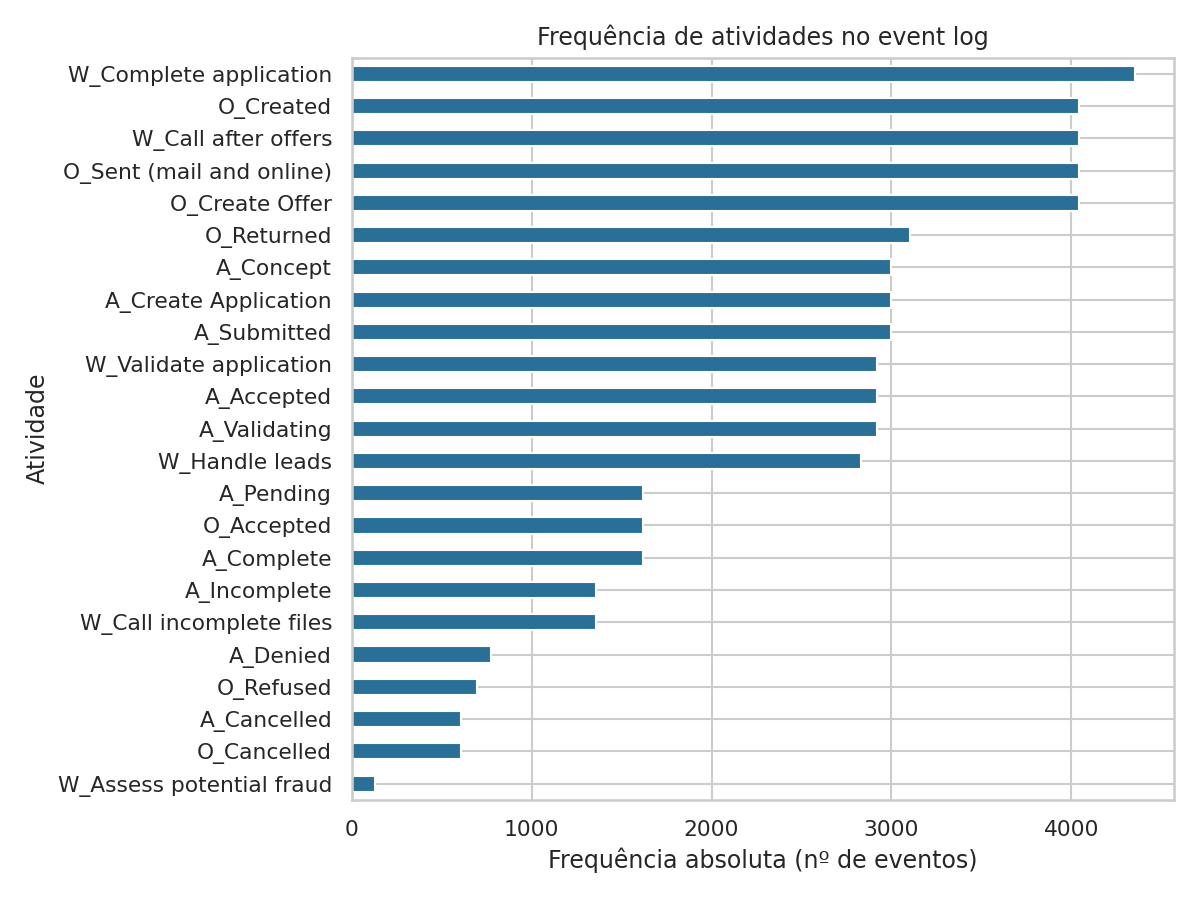
\includegraphics[width=0.48\textwidth]{01_activity_frequency.png}\hfill
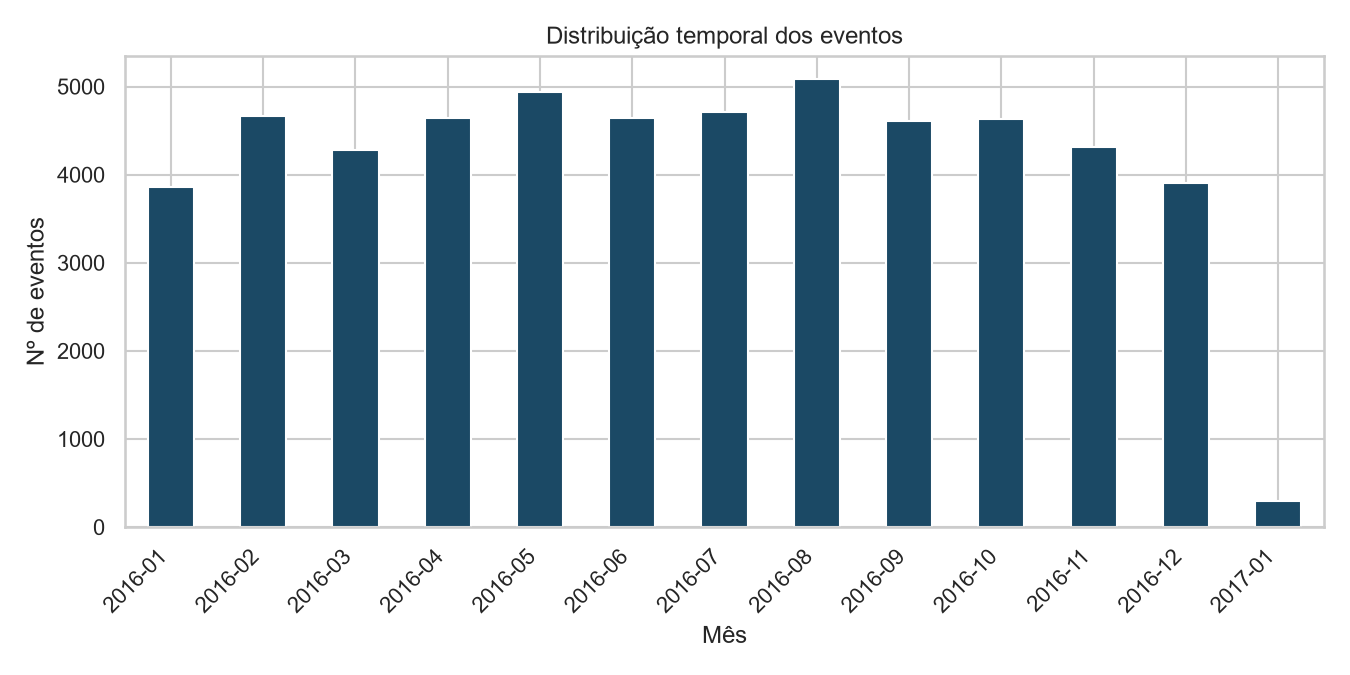
\includegraphics[width=0.48\textwidth]{02_temporal_distribution.png}
\caption{Frequência de atividades (esq.) e distribuição temporal dos eventos (dir.).}
\label{fig:eda1}
\end{figure}

\begin{figure}[H]
\centering
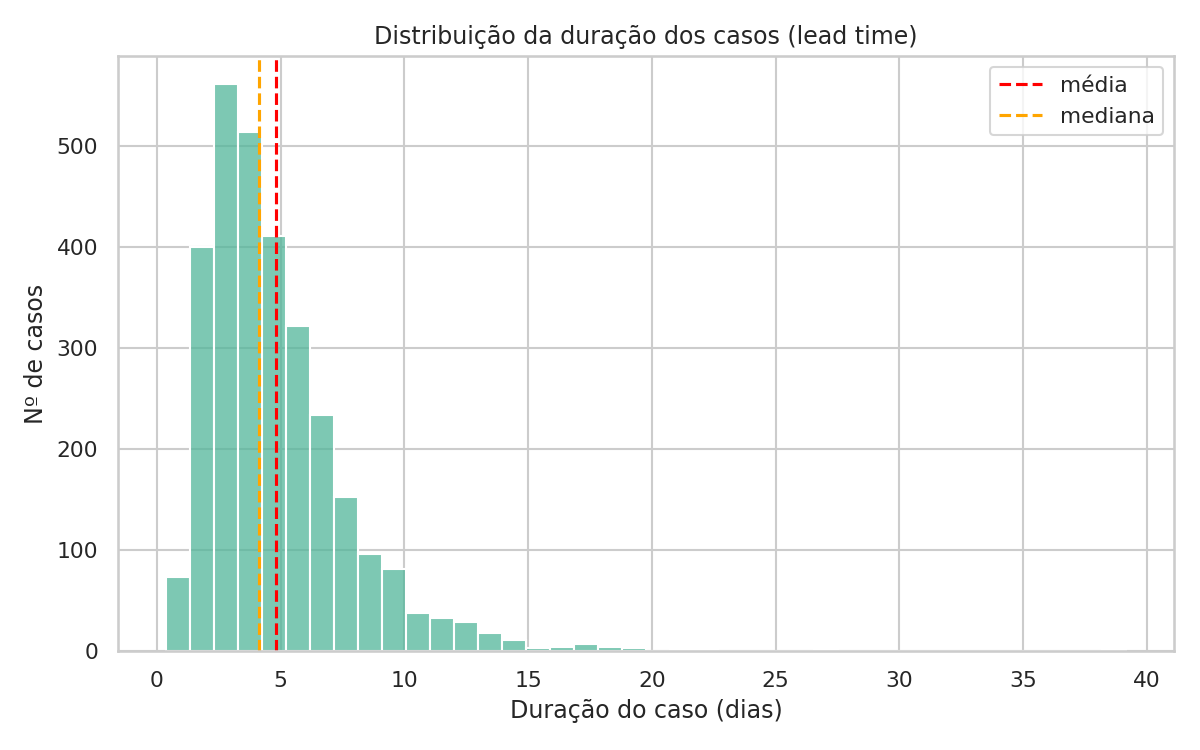
\includegraphics[width=0.62\textwidth]{03_case_duration_distribution.png}
\caption{Distribuição da duração dos casos (\textit{lead time}).}
\label{fig:duracao}
\end{figure}

Todos os casos iniciam por \texttt{A\_Create Application} (100\%). Os desfechos finais
são: \texttt{A\_Complete} (1.621 casos, 54,0\%), \texttt{A\_Denied} (772, 25,7\%) e
\texttt{A\_Cancelled} (607, 20,2\%). Foram identificadas \textbf{169 variantes} distintas:
a variante mais frequente cobre 19,33\% dos casos e as cinco primeiras somam 44,47\%
--- estrutura de cauda longa típica de processos com laços e ramificações condicionais.

\begin{figure}[H]
\centering
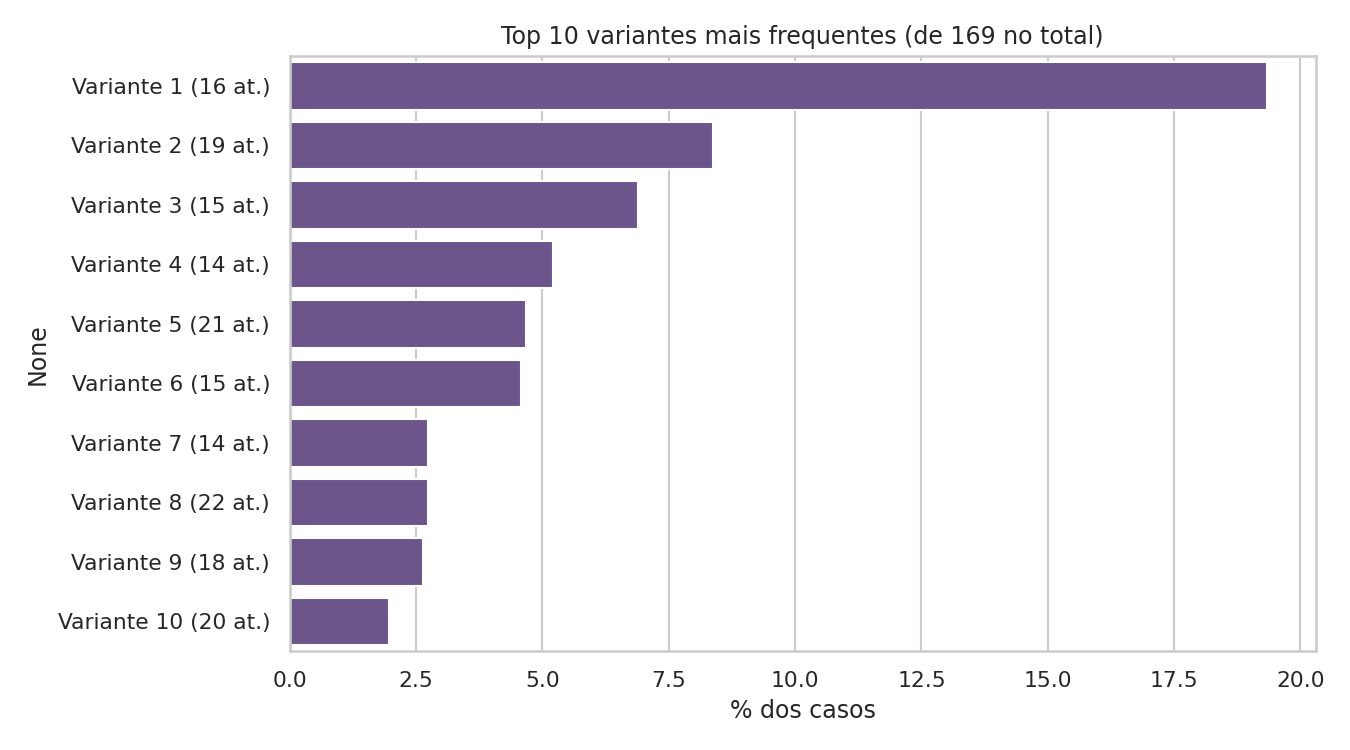
\includegraphics[width=0.65\textwidth]{05_top_variants.png}
\caption{Top 10 variantes mais frequentes (de 169 no total).}
\label{fig:variantes}
\end{figure}

\subsection{Process Discovery}

O DFG completo (Figura~\ref{fig:dfg}, esq.) revela alta conectividade entre atividades.
Ao filtrar arestas com frequência inferior a 10\% da máxima (dir.), obtém-se uma
visualização mais legível do \textit{happy path} --- equivalente conceitual ao Heuristic
Miner.

\begin{figure}[H]
\centering
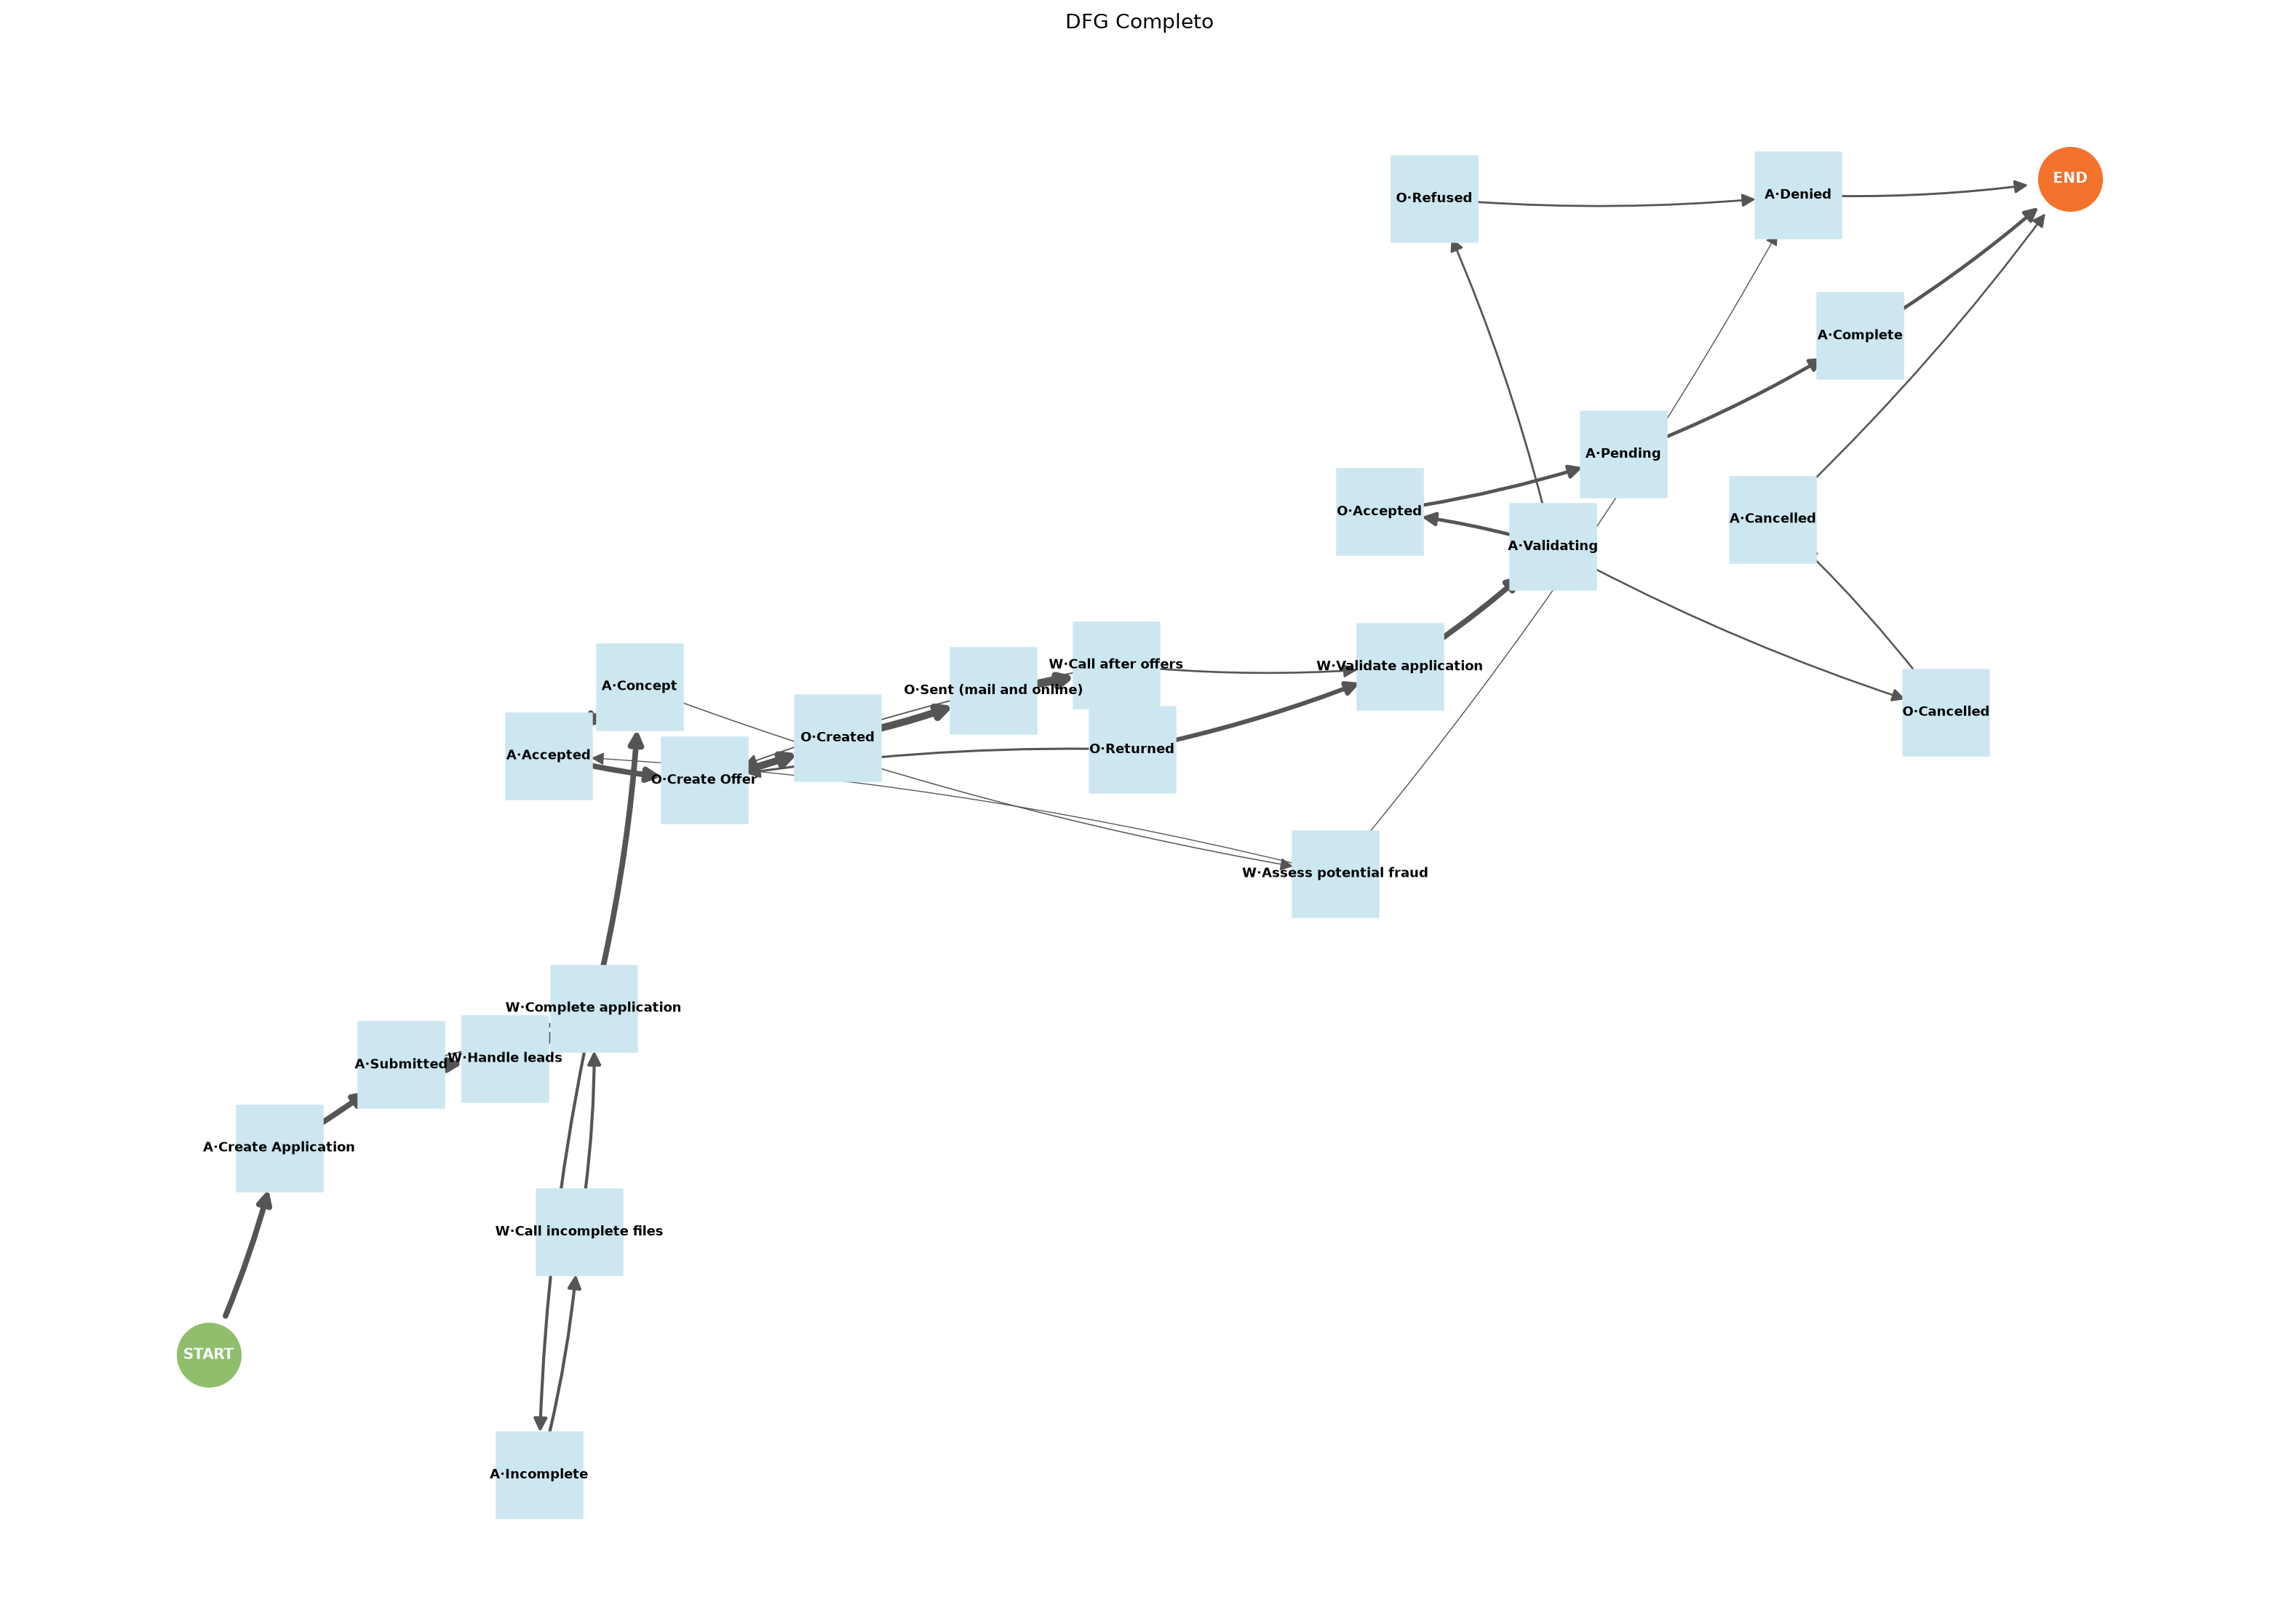
\includegraphics[width=0.82\textwidth]{06_dfg_full.png}\\[6pt]
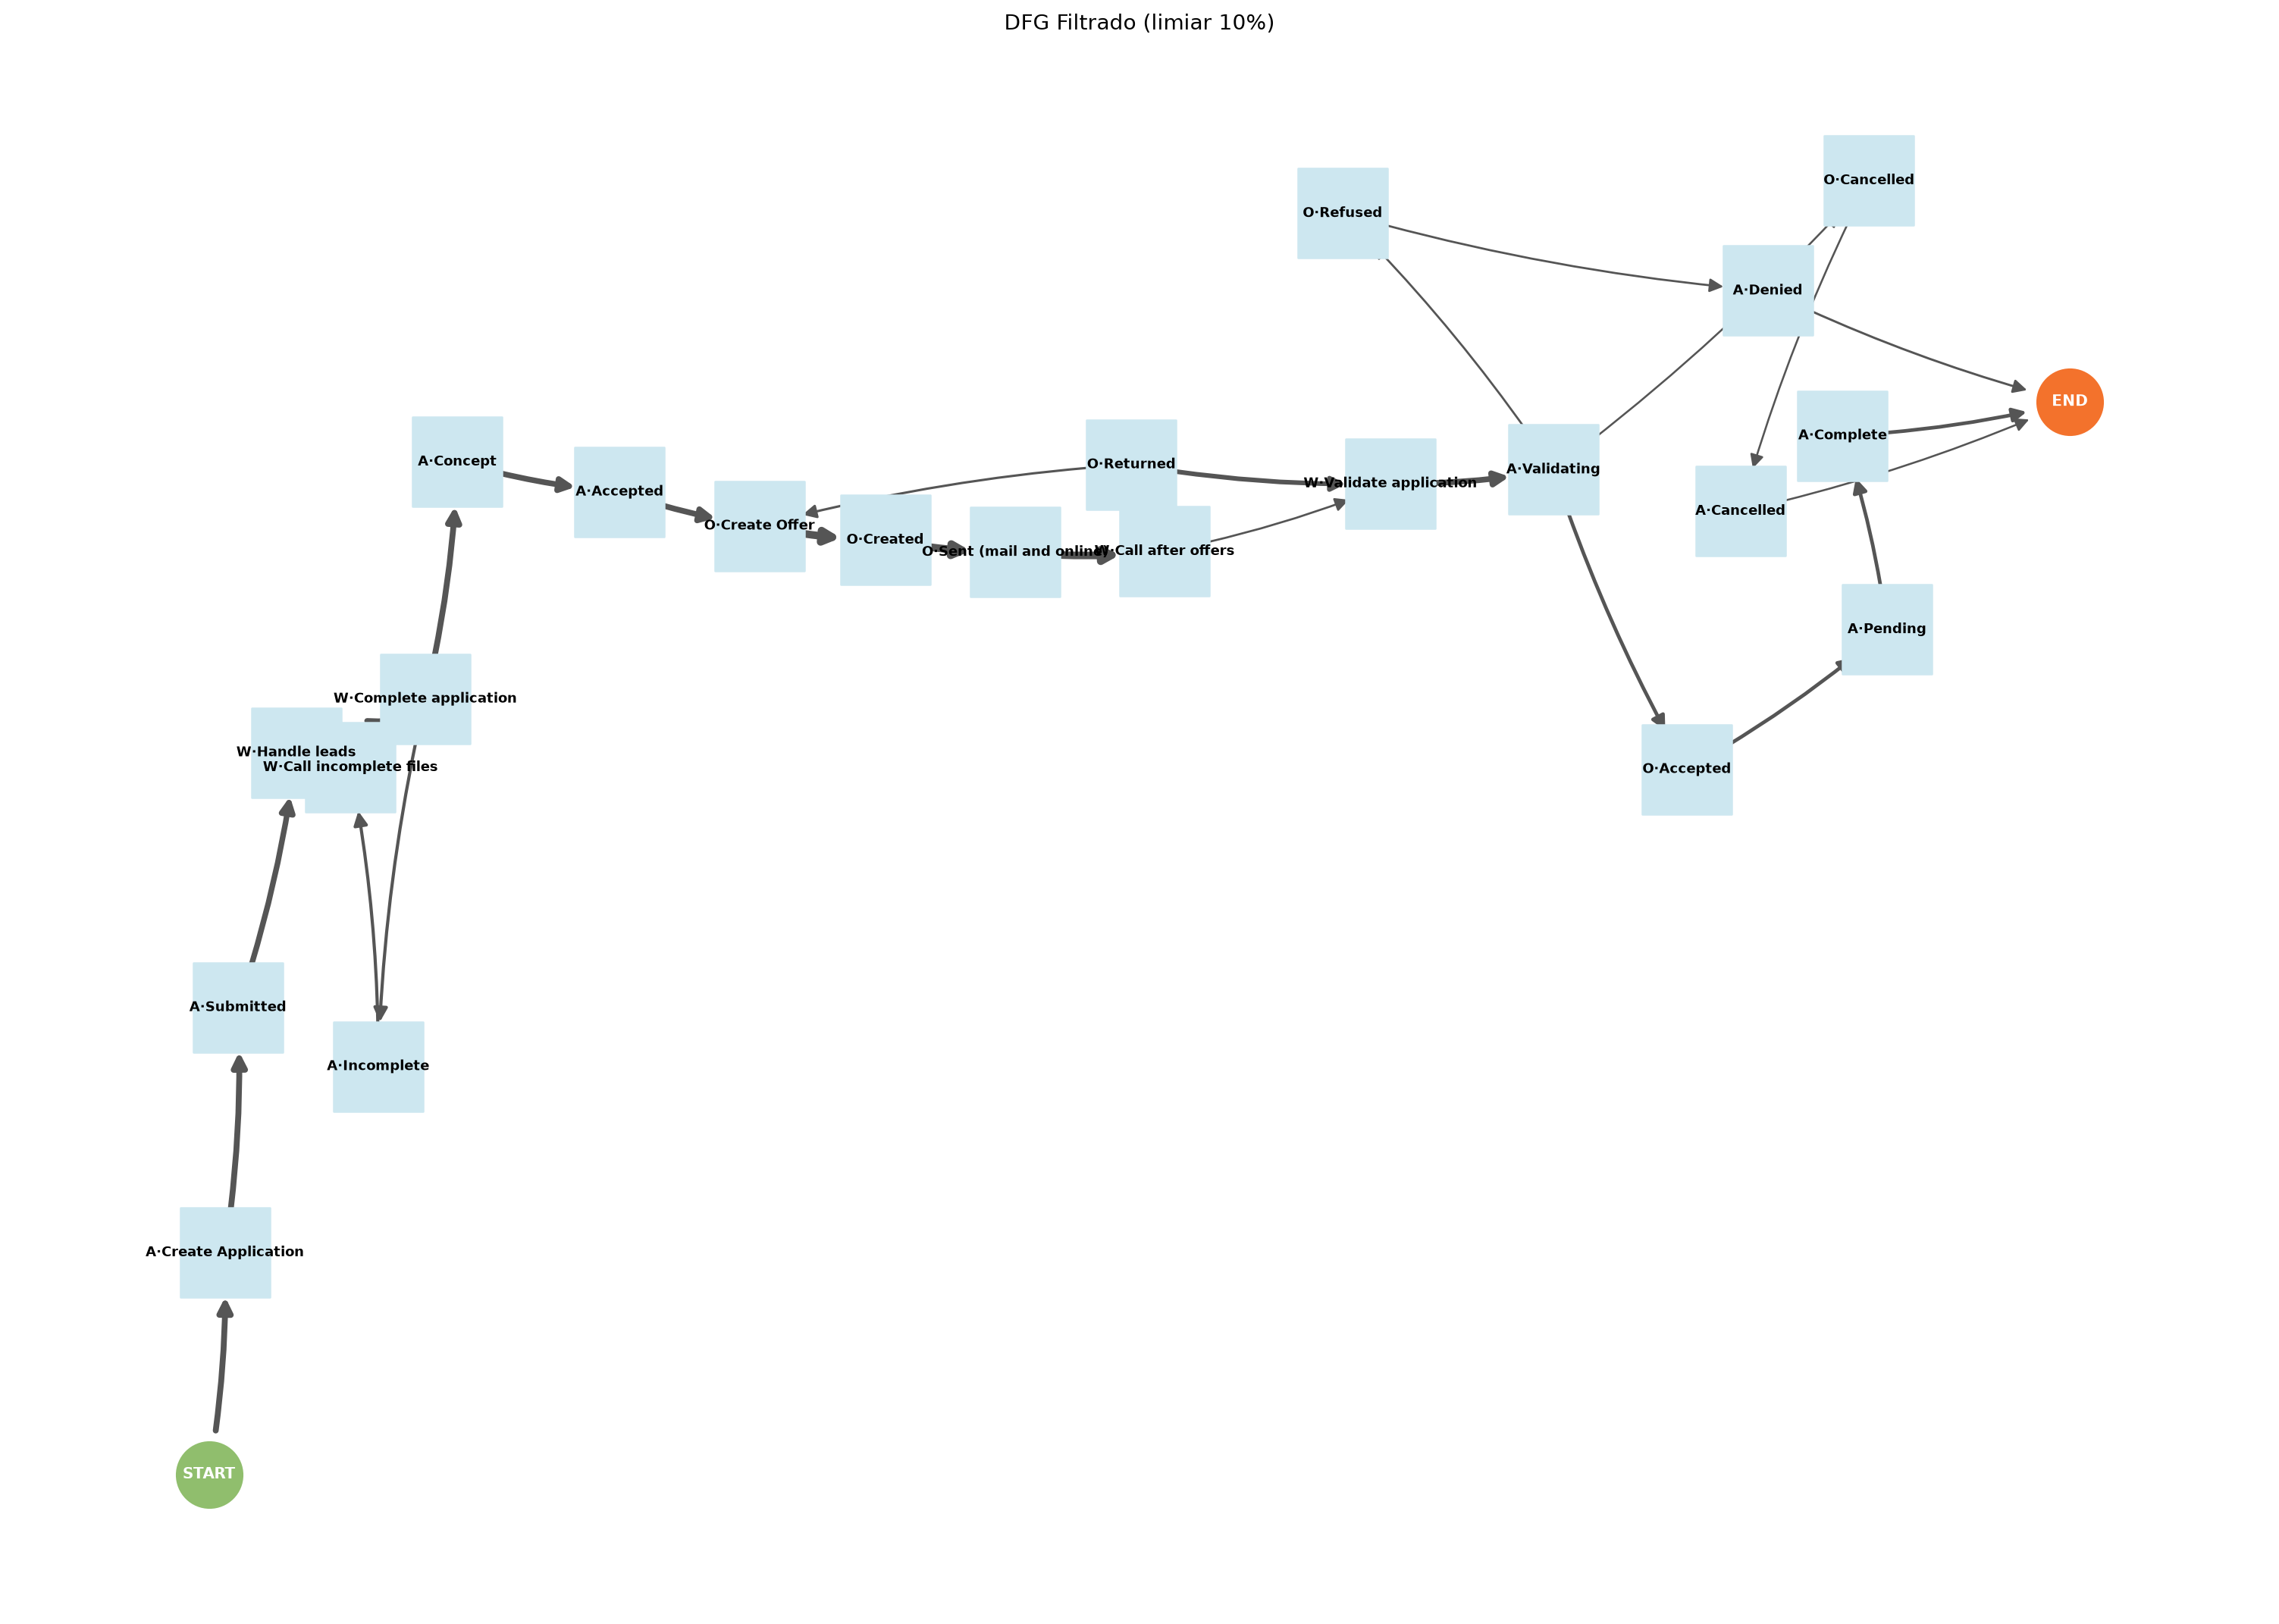
\includegraphics[width=0.82\textwidth]{07_dfg_filtered_heuristic.png}
\caption{DFG completo (acima) e DFG filtrado com limiar de 10\% (abaixo).}
\label{fig:dfg}
\end{figure}

O Alpha Miner descobriu uma rede de Petri com 23 \textit{places} para 23 transições. O
número elevado de \textit{places} é consistente com a literatura sobre as limitações do
algoritmo diante de laços de re-trabalho e múltiplas ofertas.

\begin{figure}[H]
\centering
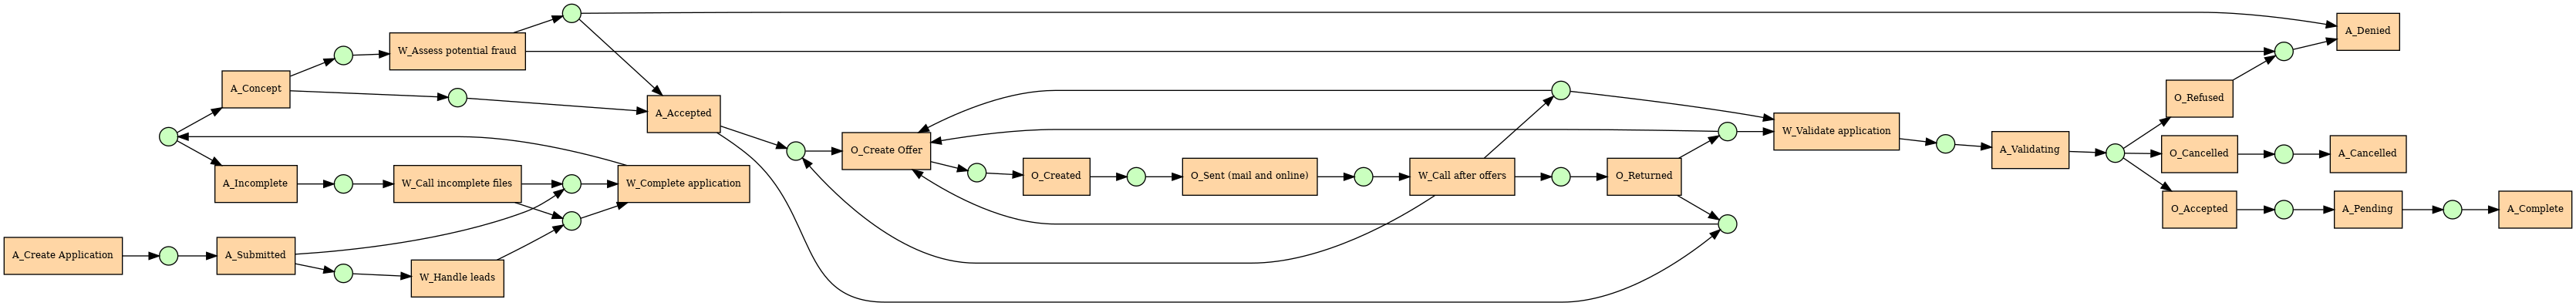
\includegraphics[width=0.95\textwidth]{08_alpha_miner_net.png}
\caption{Rede de Petri descoberta pelo Alpha Miner.}
\label{fig:alpha}
\end{figure}

O Inductive Miner não identificou cortes estruturais limpos para a maioria das atividades
após as três primeiras etapas sequenciais, recorrendo ao modelo flor --- resultando em
uma process tree com 23 folhas, na qual um único nó de loop engloba praticamente todo
o vocabulário de atividades restante. Esse resultado, por si só, é informativo: revela que
o processo possui variabilidade estrutural maior do que um modelo sequencial idealizado
capturaria.

\subsection{Conformance Checking}
\label{sec:resultados_conf}

\begin{table}[H]
\centering
\caption{Métricas de conformidade por algoritmo de descoberta.}
\label{tab:conformance}
\begin{tabularx}{\textwidth}{Xrrrrr}
\toprule
\textbf{Modelo} & \textbf{Fitness} & \textbf{Precision} & \textbf{Generaliz.} & \textbf{Simplicity} & \textbf{Arestas} \\
\midrule
DFG filtrado (Heuristic-like) & 0,9893 & 1,0000 & 1,0000 & 0,9149 &  24 \\
Alpha Miner                   & 1,0000 & 1,0000 & 1,0000 & 0,9058 &  29 \\
Inductive Miner               & 0,9973 & 0,0664 & 0,0664 & 0,1938 & 422 \\
DFG completo (bruto)          & 1,0000 & 1,0000 & 1,0000 & 0,9058 &  29 \\
\bottomrule
\end{tabularx}
\end{table}

\begin{figure}[H]
\centering
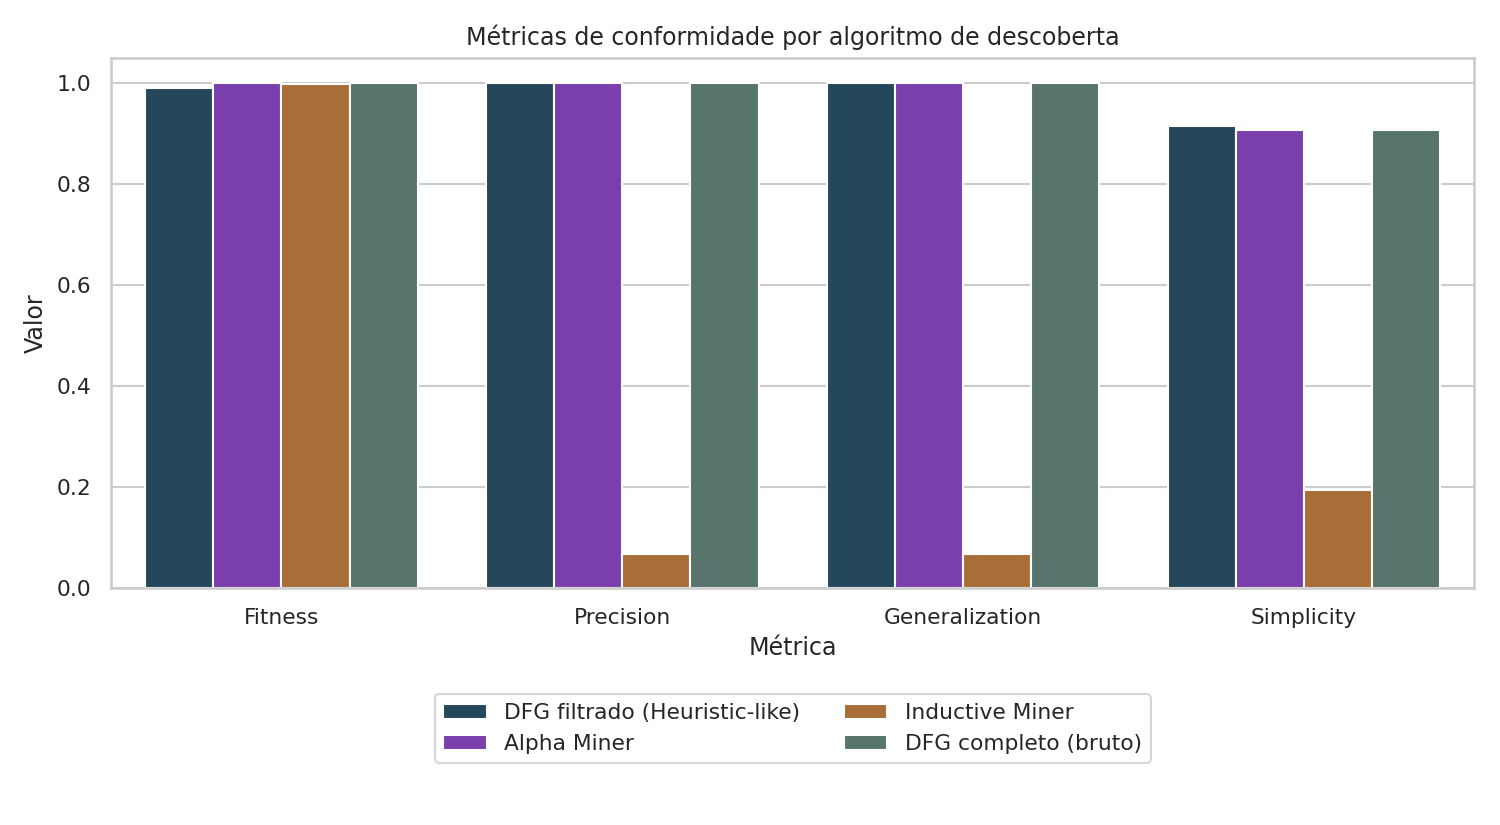
\includegraphics[width=0.56\textwidth]{09_conformance_metrics.png}\hfill
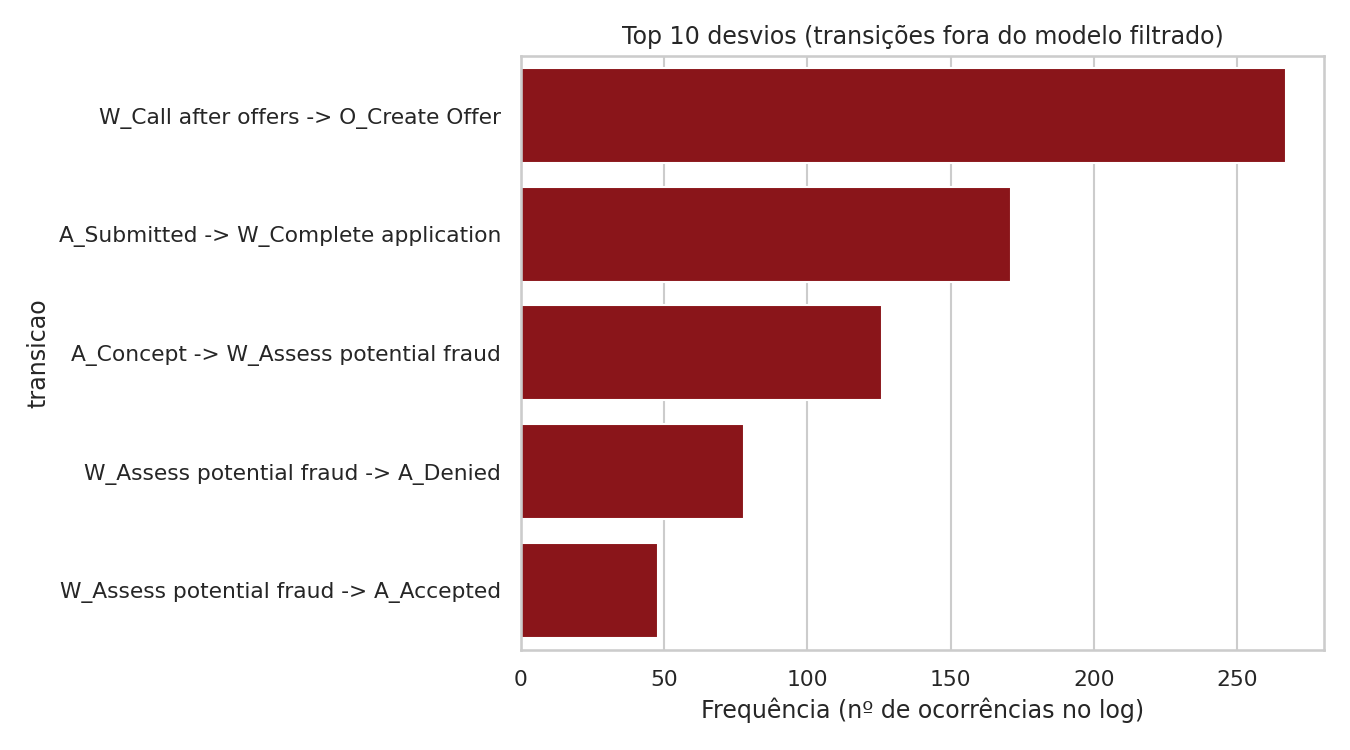
\includegraphics[width=0.40\textwidth]{10_top_deviations.png}
\caption{Métricas de conformidade por modelo (esq.) e top desvios contra o DFG filtrado (dir.).}
\label{fig:conformance}
\end{figure}

O resultado mais relevante é o trade-off exibido pelo Inductive Miner: fitness de 0,9973
mas precisão de apenas 0,0664 --- assinatura clássica do modelo flor, que com 422
arestas permite combinações jamais observadas no log. Os cinco principais desvios
identificados contra o DFG filtrado são listados na Tabela~\ref{tab:desvios}:

\begin{table}[H]
\centering
\caption{Top 5 desvios identificados contra o modelo DFG filtrado.}
\label{tab:desvios}
\begin{tabularx}{\textwidth}{Xr}
\toprule
\textbf{Transição (desvio)} & \textbf{Frequência} \\
\midrule
\texttt{W\_Call after offers} $\to$ \texttt{O\_Create Offer}         & 267 \\
\texttt{A\_Submitted} $\to$ \texttt{W\_Complete application}         & 171 \\
\texttt{A\_Concept} $\to$ \texttt{W\_Assess potential fraud}         & 126 \\
\texttt{W\_Assess potential fraud} $\to$ \texttt{A\_Denied}          &  78 \\
\texttt{W\_Assess potential fraud} $\to$ \texttt{A\_Accepted}        &  48 \\
\bottomrule
\end{tabularx}
\end{table}

Os dois primeiros desvios --- laço de múltiplas ofertas e omissão eventual de
\texttt{W\_Handle leads} --- são estruturalmente esperados pelo desenho do processo.
Os três remanescentes correspondem à ramificação de análise de fraude, uma via de
exceção rara porém processualmente distinta.

\subsection{Performance Analysis}

\begin{table}[H]
\centering
\caption{Top 6 gargalos: maior tempo médio de espera entre atividades consecutivas.}
\label{tab:bottlenecks}
\begin{tabularx}{\textwidth}{Xrrrr}
\toprule
\textbf{Transição} & \textbf{Ocorrências} & \textbf{Média (d)} & \textbf{Mediana (d)} & \textbf{P90 (d)} \\
\midrule
O\_Sent $\to$ W\_Call after offers           & 4.041 & 1,27 & 0,85 & 2,70 \\
O\_Returned $\to$ W\_Validate application    & 2.252 & 1,10 & 0,73 & 2,27 \\
W\_Call after offers $\to$ W\_Validate app.  &   670 & 1,07 & 0,69 & 2,27 \\
A\_Incomplete $\to$ W\_Call incomplete files & 1.355 & 0,85 & 0,56 & 1,78 \\
W\_Call incomplete $\to$ W\_Complete app.    & 1.355 & 0,76 & 0,50 & 1,58 \\
W\_Handle leads $\to$ W\_Complete app.       & 2.829 & 0,75 & 0,48 & 1,62 \\
\bottomrule
\end{tabularx}
\end{table}

\begin{figure}[H]
\centering
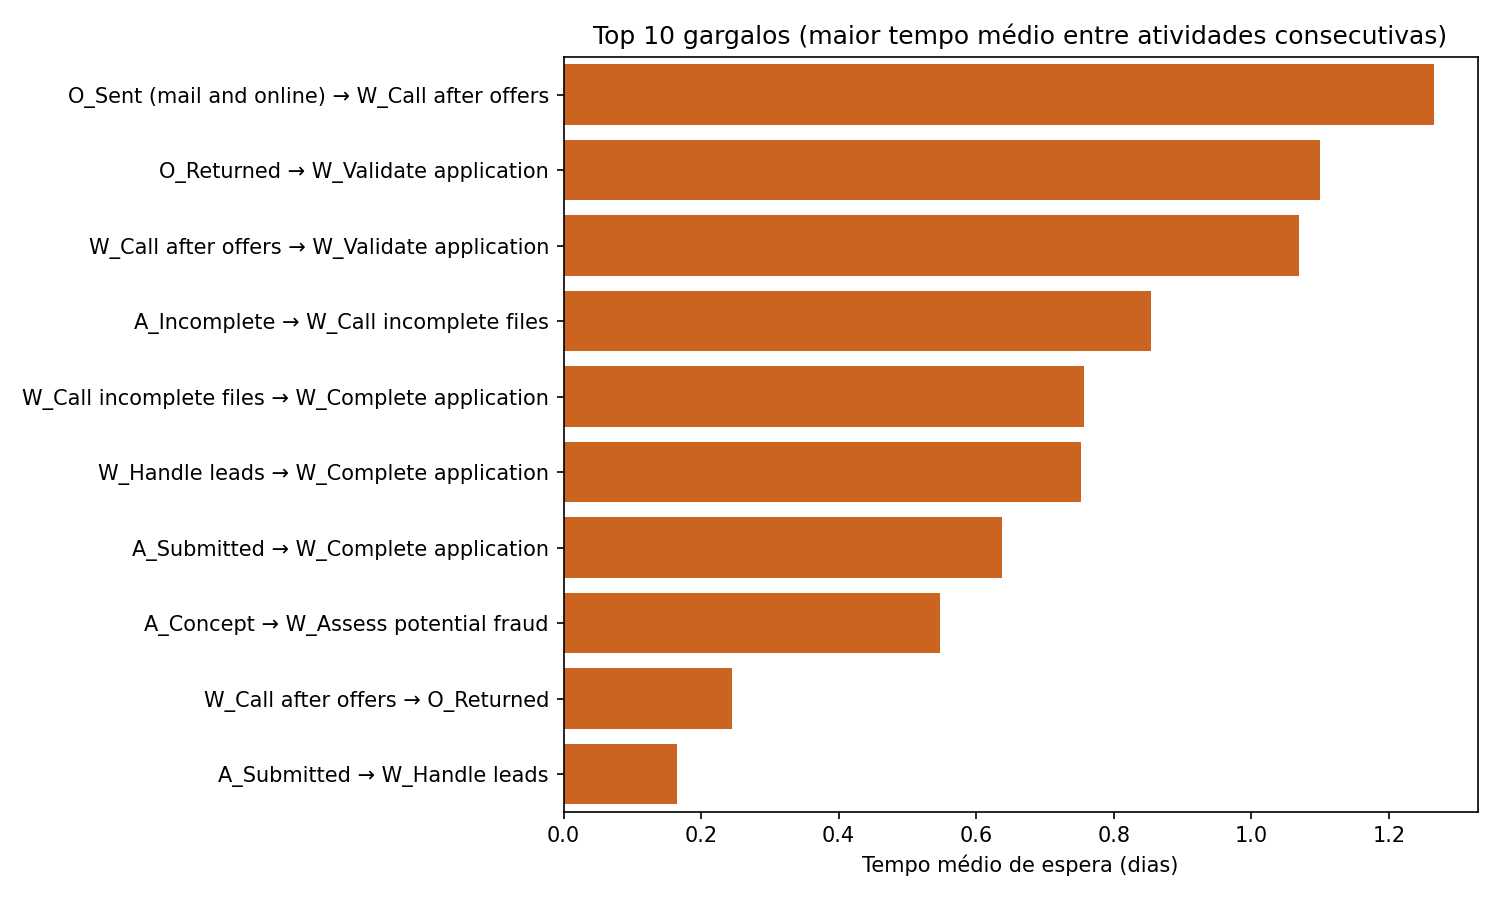
\includegraphics[width=0.56\textwidth]{11_bottlenecks.png}\hfill
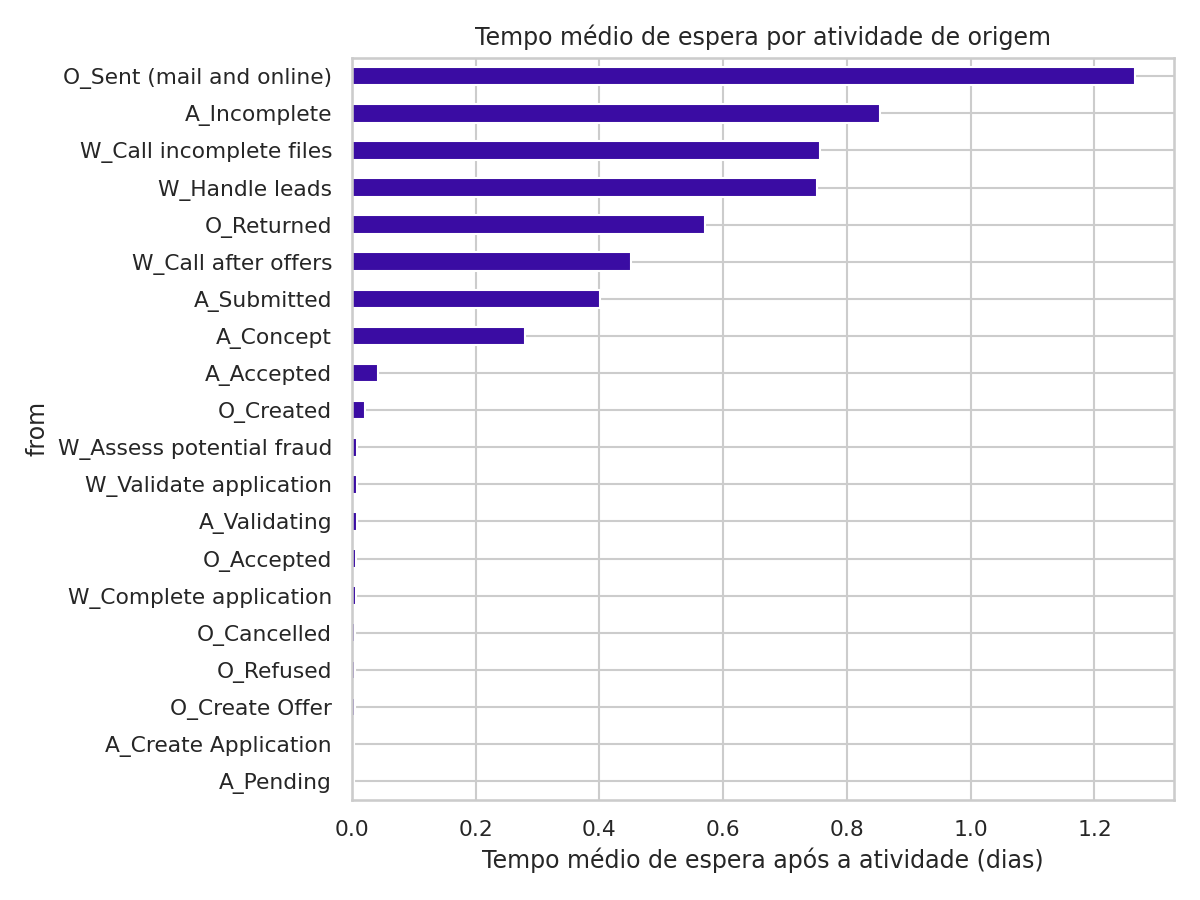
\includegraphics[width=0.40\textwidth]{12_wait_by_activity.png}
\caption{Top 10 gargalos (esq.) e tempo médio de espera por atividade de origem (dir.).}
\label{fig:bottlenecks}
\end{figure}

O maior gargalo é a transição \texttt{O\_Sent (mail and online)} $\to$
\texttt{W\_Call after offers} (média 1,27~d, mediana 0,85~d, P90 2,70~d). As etapas
automáticas (\texttt{A\_Submitted}, \texttt{O\_Created}) apresentam tempos quase nulos
--- evidenciando que o gargalo reside na capacidade de atendimento humano, não na
tecnologia.

% ===========================================================
\section{Discussão}
% ===========================================================

\subsection{Síntese frente às perguntas norteadoras}

\begin{itemize}
  \item \textbf{Processo real vs. esperado:} o \textit{happy path} é seguido por apenas
        19,3\% dos casos; os demais divergem via laços de re-trabalho ou ramificação de
        fraude, gerando 169 variantes --- o processo real é substancialmente mais variável
        do que um fluxograma idealizado sugeriria.
  \item \textbf{Principais gargalos:} concentram-se nas etapas de contato pós-oferta e
        validação documental (\texttt{O\_Sent} $\to$ \texttt{W\_Call after offers},
        \texttt{O\_Returned} $\to$ \texttt{W\_Validate application}), ambas dependentes
        de ação humana, com tempos médios superiores a 25 horas.
  \item \textbf{Desvios mais frequentes:} laço de múltiplas ofertas, omissão de
        \texttt{W\_Handle leads} e ramificação de análise de fraude.
  \item \textbf{Conformidade:} as quatro métricas evidenciam o trade-off fitness $\times$
        precision do Inductive Miner, com assinatura clássica do modelo flor (fitness alta,
        precisão 0,07, 422 arestas permitidas).
\end{itemize}

\subsection{Alpha Miner vs. Inductive Miner}

Considerando métricas de conformidade e interpretabilidade, o Alpha Miner produziu
neste log representação mais equilibrada: fitness e precisão elevadas com 29 arestas
compatíveis com a complexidade real do processo. O Inductive Miner, apesar de
robustez teórica superior (garante \textit{soundness} da rede resultante), foi prejudicado
pela alta variabilidade comportamental: não encontrando cortes estruturais limpos,
recorreu ao modelo flor, sacrificando precisão e simplicidade em favor de fitness. Esse
resultado ilustra o ponto consolidado por \cite{leemans2013}: a qualidade do Inductive
Miner depende fortemente da estruturação comportamental do log --- processos com alta
variabilidade \textit{ad-hoc} tendem a produzir modelos flor de baixo valor analítico.

% ===========================================================
\section{Limitações}
\label{sec:limitacoes}
% ===========================================================

\subsection{Limitações do dataset}

\begin{itemize}
  \item A indisponibilidade de internet impediu o uso do BPI17 real e do PM4Py, obrigando
        ao log sintético, que não captura o ruído idiossincrático, outliers e anomalias
        genuínas do log real.
  \item Toda variabilidade do log sintético foi programada explicitamente (laços, ramificação
        de fraude, número de ofertas), diferentemente de um log real, onde a variabilidade
        emerge de comportamento organizacional não documentado.
  \item O volume do log sintético (3.000 casos) é fração do real ($\sim$31.509 casos),
        podendo afetar a robustez estatística de métricas sensíveis ao tamanho da amostra.
\end{itemize}

\subsection{Limitações dos algoritmos de descoberta}

\begin{itemize}
  \item O Alpha Miner não trata adequadamente loops curtos, construtos de escolha
        não-livre e ruído \cite{vanderAalst2004}.
  \item O Inductive Miner simplificado (sem podas de ruído como nas variantes IMf/IMlc)
        recorreu ao modelo flor diante da alta variabilidade do log.
  \item O Heuristic Miner não foi implementado como algoritmo independente; foi
        aproximado por DFG filtrado por frequência, sem as heurísticas de dependência
        estatística do algoritmo original (\textit{dependency measure}).
\end{itemize}

\subsection{Limitações da análise de conformidade}

\begin{itemize}
  \item As métricas foram implementadas como aproximações heurísticas (\textit{replay}
        de arestas e proxies de \textit{escaping edges}), não como os algoritmos de
        \textit{token replay} ou \textit{alignments} do PM4Py --- os valores numéricos
        não são diretamente comparáveis com benchmarks da literatura.
  \item A comparação entre o modelo do Alpha Miner e o log apresenta grau de
        circularidade metodológica (mitigado pela inclusão do Inductive Miner com semântica
        independente, conforme Seção~\ref{sec:circular}).
\end{itemize}

\subsection{Ameaças à validade e trabalhos futuros}

Os resultados quantitativos específicos refletem os parâmetros do gerador sintético e não
devem ser generalizados como descrição do processo real do BPI17. Como trabalho
futuro, recomenda-se: (i)~reexecutar a metodologia sobre o dataset real tão logo haja
acesso à internet; (ii)~utilizar o PM4Py para validar as implementações próprias;
(iii)~aplicar \textit{alignment-based conformance checking}; e (iv)~explorar o Inductive
Miner com filtragem de ruído (IMf) para obter modelos mais precisos sem recorrer ao
modelo flor.

% ===========================================================
\section{Conclusão}
% ===========================================================

Este trabalho aplicou, de ponta a ponta, uma metodologia de Process Mining sobre um
log de eventos estruturalmente fiel ao processo de empréstimos do BPI Challenge 2017,
cobrindo importação e limpeza de dados, EDA, descoberta de processo (Alpha Miner e
Inductive Miner), conformance checking (fitness, precision, generalization, simplicity) e
análise de performance e gargalos.

Os resultados mostraram um processo com 169 variantes de execução, no qual apenas
19,3\% dos casos seguem o caminho idealizado, e cujos principais pontos de atraso se
concentram em etapas de trabalho manual (contato pós-oferta e validação documental),
com tempos médios de espera superiores a 25 horas. A comparação entre algoritmos
evidenciou o clássico trade-off fitness $\times$ precision: o Inductive Miner obteve fitness
quase perfeita (0,997) às custas de precisão muito baixa (0,066), enquanto o Alpha
Miner produziu modelo mais equilibrado e interpretável para este caso específico.

Do ponto de vista metodológico, a principal contribuição foi demonstrar que, mesmo sem
acesso a bibliotecas especializadas como o PM4Py e sem acesso ao dataset original, é
possível conduzir de forma criteriosa e cientificamente honesta um pipeline completo de
process mining --- desde que as limitações sejam explicitamente reconhecidas e
discutidas, como feito na Seção~\ref{sec:limitacoes}.

% ===========================================================
% REFERÊNCIAS
% ===========================================================
\newpage
\renewcommand{\refname}{Referências}
\begin{thebibliography}{99}

\bibitem{medeiros2007}
ALVES DE MEDEIROS, A. K.; WEIJTERS, A. J. M. M.; VAN DER AALST, W. M. P\@.
Genetic process mining: an experimental evaluation.
\textit{Data Mining and Knowledge Discovery}, v.~14, n.~2, p.~245--304, 2007.

\bibitem{caro2019}
CARO, A. et al.
Process mining for capturing variability in production processes.
In: \textit{International Conference on Business Process Management}, 2019.

\bibitem{manifesto2011}
IEEE TASK FORCE ON PROCESS MINING\@.
Process Mining Manifesto.
In: \textit{Business Process Management Workshops}.
Lecture Notes in Business Information Processing, v.~99. Berlin: Springer, 2011.

\bibitem{leemans2013}
LEEMANS, S. J. J.; FAHLAND, D.; VAN DER AALST, W. M. P\@.
Discovering block-structured process models from event logs: a constructive approach.
In: \textit{International Conference on Applications and Theory of Petri Nets and
Concurrency}, 2013. Lecture Notes in Computer Science, v.~7927.
Berlin: Springer, p.~311--329, 2013.

\bibitem{pm4py}
PM4PY\@.
\textit{Process Mining for Python --- Documentation}.
Fraunhofer Institute / Process Intelligence, [s.d.].
Disponível em: \url{https://pm4py.fit.fraunhofer.de/}.
Acesso em: jun.~2026.

\bibitem{vanderAalst2016}
VAN DER AALST, W. M. P\@.
\textit{Process Mining: Data Science in Action}.
2.~ed. Berlin: Springer, 2016.

\bibitem{vanderAalst2004}
VAN DER AALST, W. M. P.; WEIJTERS, A. J. M. M.; MARUSTER, L\@.
Workflow mining: discovering process models from event logs.
\textit{IEEE Transactions on Knowledge and Data Engineering}, v.~16, n.~9,
p.~1128--1142, 2004.

\bibitem{vanDongen2017}
VAN DONGEN, B. F\@.
BPI Challenge 2017. Eindhoven University of Technology. Dataset.
2017. Disponível em:
\url{https://doi.org/10.4121/uuid:5f3067df-f10b-45da-b98b-86ae4c7a310b}.
Acesso em: jun.~2026.

\bibitem{weijters2011}
WEIJTERS, A. J. M. M.; RIBEIRO, J. T. S\@.
Flexible heuristics miner (FHM).
In: \textit{IEEE Symposium on Computational Intelligence and Data Mining
(CIDM)}, 2011. p.~310--317.

\end{thebibliography}

\end{document}
